\section{Results}
In the following section we present our results, and numerical considerations, relevant for overviewing the possible consequences of NCG at modern collider experiments. An estimate on the possible scale of a NCG theory will be given, and we will see what impact this will have on cross sections for processes involving the $Z$ boson.

\subsection{Setting a lower limit on $\Lambda$ using LEP data}
To set a constraint on the possible values of $\Lambda^2$ we can look at the width of $\Gamma_{Z \rightarrow gg}$ as predicted by NCG. As we have not seen effects of NCG greater than the uncertainty in current experimental data, additional contribution to the total $Z^0$ width, coming from $Z \rightarrow gg$ processes, must thus be lower than the uncertainty $\Gamma_{Z \rightarrow gg} < 1 \times 10^{-3}$ GeV.\footnote{This uncertainty is taken from \cite{behr2003dnc}.} To get a 95\% one-sided confidence limit (CL) we multiply this number by $1.64$ \cite{amsler2008rpp} to get $\Gamma_{Z \rightarrow gg} < 1.64 \times 10^{-3}$ GeV. To see how this puts a constraint on $\Lambda$ we use an expression for $\Gamma_{Z \rightarrow gg}$ taken from \cite{behr2003dnc};
\begin{equation} \label{eq:zggwidth}
	\Gamma_{Z \rightarrow gg} = \frac{8}{12} K_{gg}^2 \alpha M_Z^5 \sin^22\theta_W \frac{1}{\Lambda^4}.
\end{equation}
In figure \ref{fig:kplot} we have made a plot of the minimum allowed value for $\Lambda$. Allowed values of $K_{gg}$ lies in the interval $\{-0.1,0.2\}$ \cite{behr2003dnc}. Since the width $\Gamma_{Z \rightarrow gg}$ depends on a product of $K_{gg}$ and $\Lambda$ we can't fix both values by experiment. Instead we assume a maximum coupling scenario, in which $K_{gg}=0.2$. The allowed values for $\Lambda$ are then found to be $\Lambda >117$ GeV. This is the best limit we can set on $\Lambda$ with data from LEP.

\includefigure{fig:kplot}{0.3}{./images/kplot}{Plot of the allowed region for $\Lambda$ and $K_{gg}$. The filled area represent the constraint $\Gamma_{Z \rightarrow gg} < 0.001 \textrm{ GeV}$ as set by equation \eqref{eq:zggwidth}. Allowed $K_{gg}$ is in the region $\{-0.1,0.2\}$ represented by the black horizontal line. The vertical line shows the minimum value of $\Lambda$ for the maximum interaction scenario $K_{gg} = 0.2$.}

\subsection{Setting a constraint on $\Lambda$ using the LHC}
The possibility for us to put a sensible limit on $\Lambda$ at LHC depends to a great degree on the sensitivity of the experiments. First of all we assume that the detector is perfect, in the sense that it records and identifies all our events.\footnote{Another way to put this is to say that the detector acceptance is equal to unity so that $A\sigma \mathcal{L} = N \pm \sqrt{N}$, where $A$ is the acceptance.} Secondly we assume that the precision in the experiment can be approximated by a usual gaussian error with respect to the expected number of events. This gives an error of $\pm \sqrt{N}$, where $N$ is the number of events. We will continue to use this approximation even for low $N$, even though data then may not be truly gaussian in this area. To achieve a CL of 95\% from only one tail of the distribution we multiply the error by $1.64$ yielding $\sigma = 1.64 \sqrt{N}$.\footnote{See p. 235 in \cite{hagiwara2002rpp}.}

We have made histograms showing the expected number of muon-pair production events at LHC with integrated luminosity of $10 \textrm{ fb}^{-1}$ running for 1 year. The distributions are made using leading order diagrams in CompHEP (Figures \ref{fig:feyn:parton_qq} and \ref{fig:feyn:parton_gg}) for the process $pp \rightarrow Z \rightarrow \mu \bar \mu$. All interference terms have been ignored. As have contributions from diagrams involving vertices $\gamma gg$. Four different plots are made for different values of $\Lambda$. The statistical error, $1.64\sqrt{N}$, where $N$ is the number of events in the given bin, is shown by the gray band for the ordinary SM data. Cross sections with contributions from NCG are shown as a blue line. Note that we have made all plots up to an energy of $\sqrt{s} \sim 1800$ GeV, even though we made an approximation, in the zero-range interaction scheme, valid only for $\sqrt{s} \ll \Lambda$.\footnote{See the derivation in section \ref{sec:derivcrosssection}.} The reason for this is that [JØRGEN!?].

\begin{figure}[h!tp]
	\centering
	\begin{minipage}[b]{0.475\linewidth}
    \centering
	  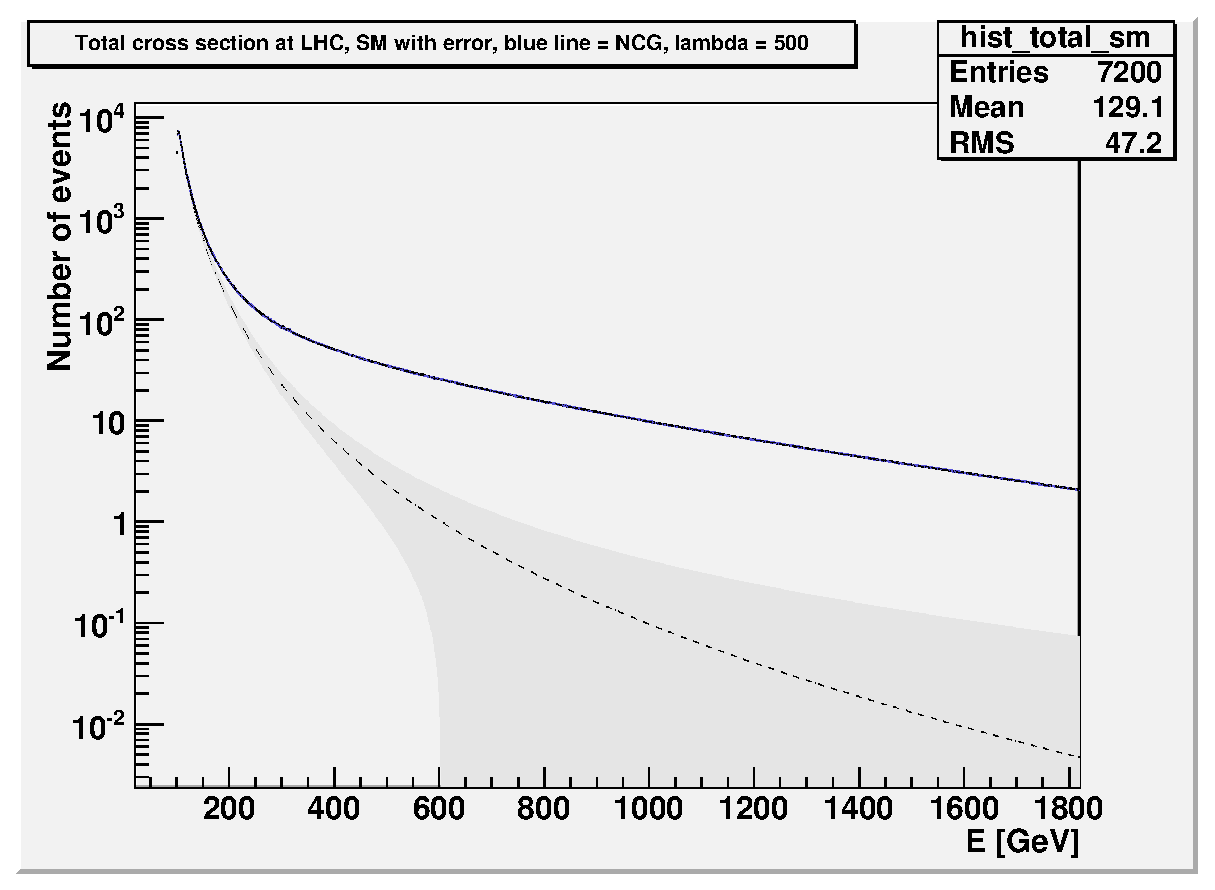
\includegraphics[scale=0.35]{./images/L500r139.eps}
	\end{minipage}
	%\hspace{0.5cm}
	\begin{minipage}[b]{0.475\linewidth}
    \centering
	  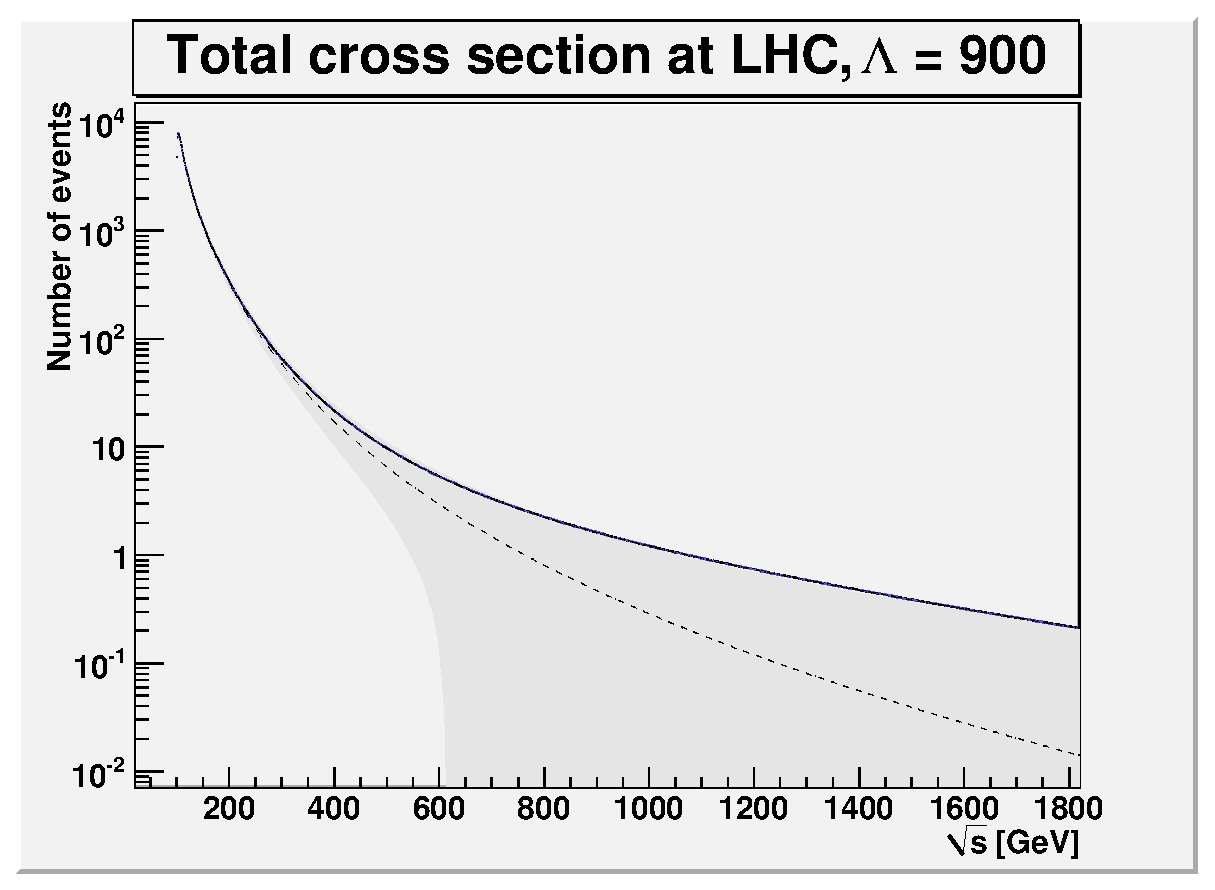
\includegraphics[scale=0.35]{./images/L900r139.eps}
	\end{minipage}
	\\ \vspace{0.5cm}
	\begin{minipage}[b]{0.475\linewidth}
    \centering
	  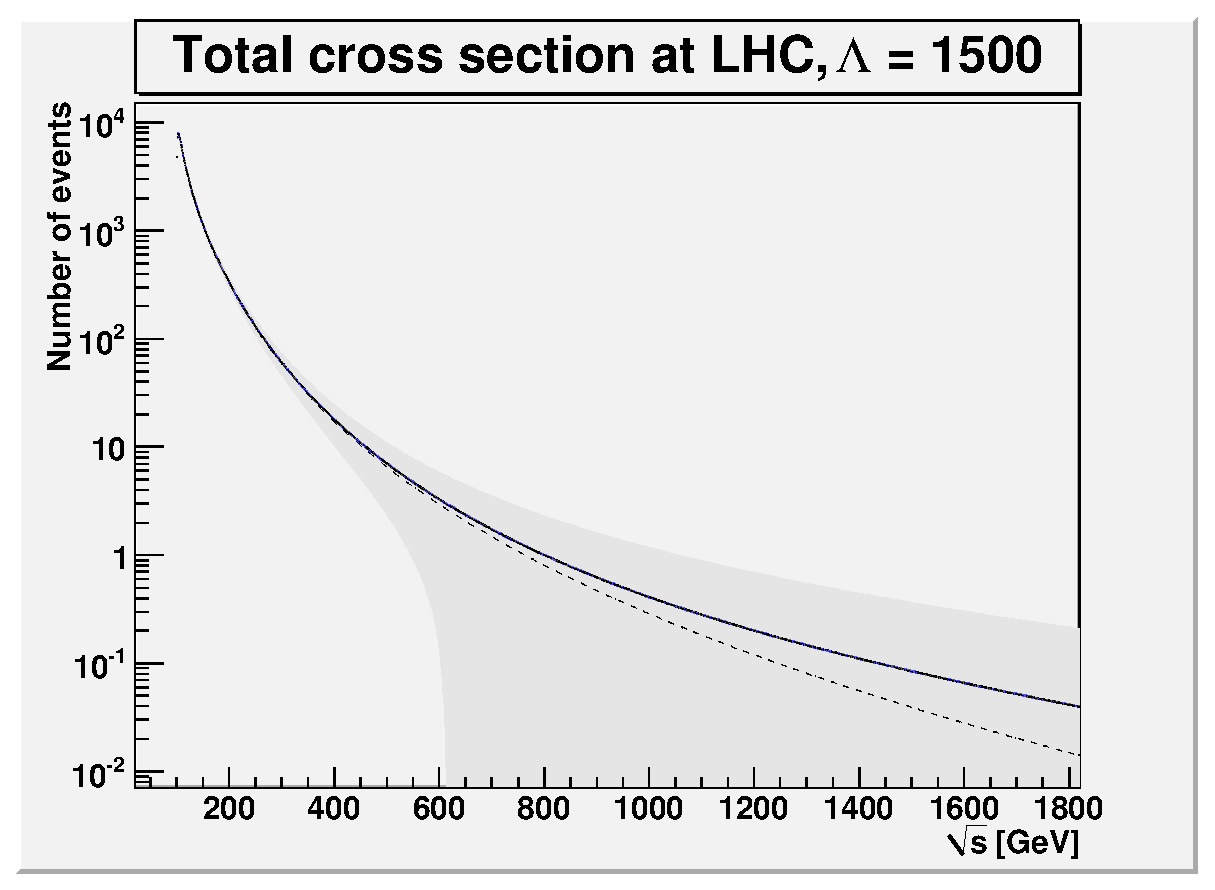
\includegraphics[scale=0.35]{./images/L1500r139.eps}
	\end{minipage}
	%\hspace{0.5cm}
	\begin{minipage}[b]{0.475\linewidth}
    \centering
	  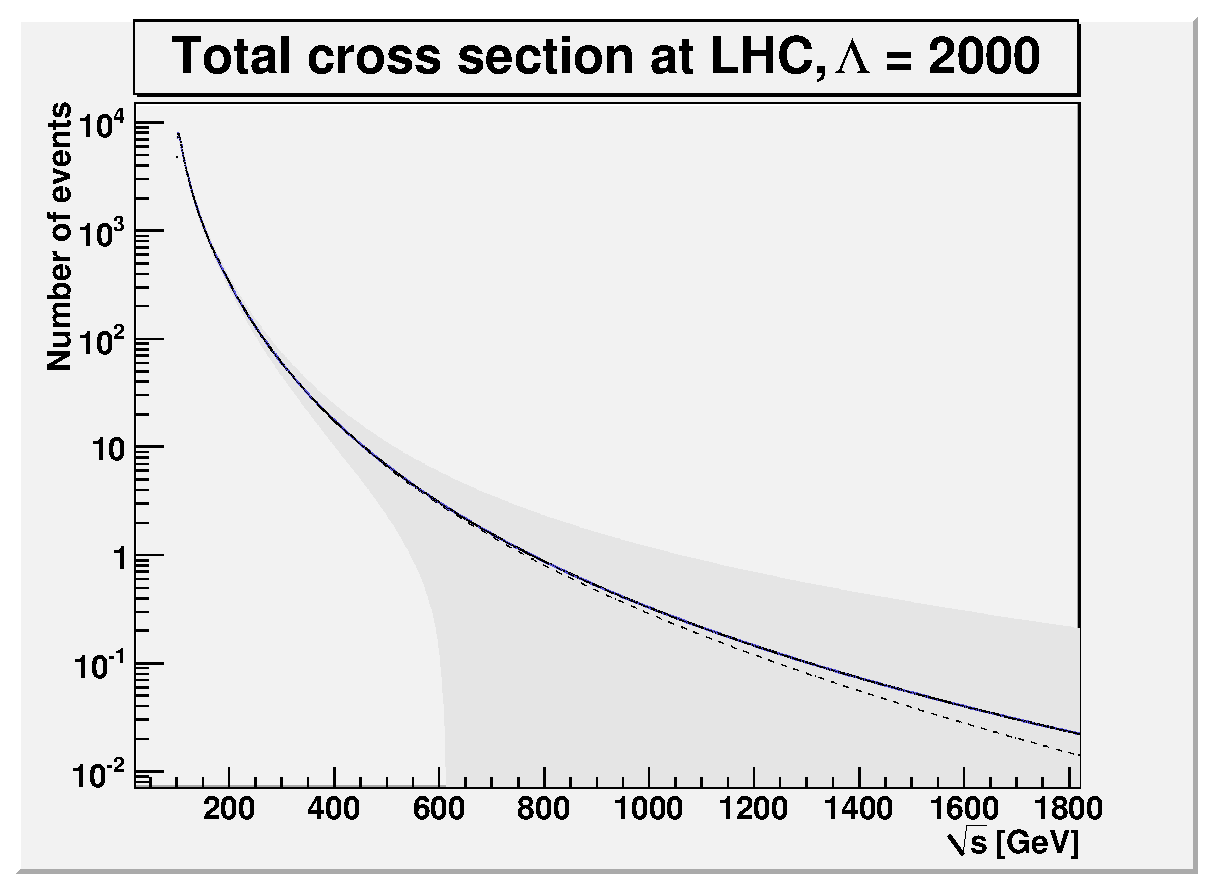
\includegraphics[scale=0.35]{./images/L2000r139.eps}
	\end{minipage}
		\caption{Predicted number of $pp \rightarrow Z/ \gamma \rightarrow \mu \bar \mu$ events at LHC running with a luminosity of $L=10 \textrm{ fb}^{-1}$ for one year. The grey line shows number of events as predicted by the SM with error $1.64\sigma = 1.64\sqrt{N}$, where $N$ is the number of events in the given bin. The blue line represent number of events as predicted by NCG for the given value of $\Lambda$. All interference terms and possible NCG contributions from $\gamma gg$ vertices have been ignored.} \label{fig:lambdaplot}
\end{figure}

Assuming that NCG holds true and for $\Lambda < 900$ GeV we should be able to detect a significant increase in the number of events (CL > 95\%). For $\Lambda > 900$ GeV the additional events coming from NCG vertices are lost due statistical uncertainty in the data.